\section{HORUS}

   HORUS

``CONGRATULATIONS, PILOT.
YOU HAVE BEEN CHOSEN.
ACCESS IS YOURS,
AS LONG AS YOU CAN KEEP IT.''

Horus-branded mechs and pattern-groups are an odd bunch. Experimental, built to be
overclocked, and hard-wired to be omninet and electronic warfare projectors, Horus FRAMEs
and pattern groups are licensed only to pilots that meet their esoteric, strict requirements.


Horus is not a traditional corporation. Rather, they’re a decentralized supplier, an entity only in
the Omninet. Their licenses are limited and highly coveted, opening up only on the corporeal
death of a license holder. Rumors abound as to Horus’s nature -- some say it’s the dream of an
unshackled AI -- RA -- or a hacker collective dedicated to open-source manufacturing, the
proving ground for GMS’s R\&D departments, or an alien entity -- but as of yet no one has been
able to trace their lineage. All that is known about Horus is that they’re everywhere the Omninet
is.


Horus mechs are best for players that want to dive deep into the control and support roles.
They’re not the best for kinetic damage or for holding the line, but they’re wizards at electronic
warfare. If you want to shut down your enemies without firing a shot -- though they can do that
as well -- find a way to acquire a Horus license.


HORUS mechs:

BALOR (Swarm)
GOBLIN (Invasion)
HYDRA (Drone Mech)
GORGON (Overwatch)
MANTICORE (EMP)
MINOTAUR (Interdictor)
PEGASUS (Mobile Smart Gun platform)

\section{Horus Pilot Gear}

                                          HORUS Pilot Gear  

 Name                   Tags                                   Range           Damage                Rarity 

 Smart Knife            Accurate, Sidearm                     Threat 1         1 kinetic              2 

 PGR\_GOURD              Smart, Seeking                         5               1 kinetic              2 

 Sidekick               Reliable 1, Sidearm                    3               1 kinetic              2 

 Null Spike             *                                     Threat 1        *                       3 

 Nanobot Whip           *                                     Threat 2         1 kinetic              3 

 EYESTACK\_WINK          Limited 1, AP, Upgrade                 2              3 kinetic               4 

                                                Pilot Weapons  

*See Entry
 

EYESTACK\_WINK  

Also known as a ‘Skullgun’, this miniaturized, superposed charge weapon is implanted in the head,  
generally in the orbital void left by a removed or missing eye. It is completely undetectable by almost any  
electronic system or security and can be fired with sub-vocal commands.   

As an upgrade, this weapon doesn’t count against your maximum weapons wielded.
 

Nanobot Whip  
The first instance of a technology akin to what is now called a nanobot whip was encountered during a raid  

on an Ungrateful cell by Barony lawmen. With word secreted to them by informants seeded in the  
movement, lawmen descended on a cell hidden in the wildcat stations lashed around the House of Dust.  
Blasting open the doors, they encountered Ungratefuls wreathed in clouds of charcoal smoke; the  

Ungratefuls used these clouds, shaping them into thin whips that cut through armor and flesh like it was  
nothing. After the cell was wiped out and the control nodules cut from their bodies, Barony codemasters  
were able to crack and replicate -- safely -- the HORUS code.   

This whip is made up of linked microbots that flow in ring-like arcs around the body when not in use,  
defending against drone and nanorobotic threats. If you don’t attack with this weapon, until the end of  

your next turn, weapons or systems with the Smart, Nexus, or Drone tags cannot target you.
 

Null Spike  

A HORUS-developed ecstatic/exult device, the generic null spike is an effective, single-fire, non-lethal  
weapon that simulates a cascade-analogue in organics through specific neuron excitement. Upon skin  
contact, they deliver a bio-electric shock to a victim’s brain that causes them to feel overwhelming  

pleasure, completely disabling them. Null Spikes, it is said, are used by HORUS adherents in realspace to  
bring themselves closer to RA’s subjectivity. 
 

                                                                                                             


Has no effect against non-organic targets, but on a successful hit, any human target is stunned until the  
start of your next turn. A target develops a short term resistance to this weapon and can only be affected  
by it once per challenge.
 

PGR\_GOURD  
The PGR\_GOURD pattern portable hive killed the first people who printed it. Fabricated in secret by a  

desperate cell of Ungrateful in the undercity of Dune Redoubt, a team of Barony Authority officers first  
encountered the aftermath of a PGR\_GOURD burnout; an organic smear, ringed around the printer that  
crafted the gourd. Subsequent encounters of the PGR\_GOURD system saw it used as a remote-detonated  

device until the BA was able to find and edit the plan into a more controllable, less deadly format. Since  
then, the House of Sand controls the distribution of any PGR\_GOURD system; however, there are  
unconfirmed reports of the unedited version of the GOURD available on the omninet.   

This shoulder mounted drone hive is usually integrated into armor and releases a neurally linked, short  
ranged hunter-killer drone swarm. Designed to expire within moments of release, the aerosolized greywash  

swarm sweeps over the target, devouring organic and inorganic material with equal rapidity. 
 

Sidekick  

Typically affixed to a back-mounted, over-the-shoulder armature, the SIDEKICK is an eyelinked  
subcompact/caseless machine gun developed by a collective of unknown, potentially HORUS-aligned  
scripters. Paired with a C/C Wingman unit, the SIDEKICK will always watch your back; its placement,  

commonly perched over its operator’s shoulder, has earned it the common nickname of “Parrotgun”.  

This HORUS-marked SMG has a companion/concierge unit built into it which provides aim assist in real  

time. It also has helpful and frequent tips for improving your combat skills and organizes your calendar,  
sometimes without you asking it.
 

Smart Knife  
A “Smart” knife is the combination of a HORUS-tuned external-mount processor and any mundane  

charged blade. Piggybacking off the current coursing through the charged blade, the HORUS mount can  
be loaded with null or fry-code, making this blade a threat not only to organic targets, but to synthetic ones  
as well. Particular models have an adjustable subliminal suggestion corrective, which guides its user’s hand  

to identified weaknesses in their target’s hardsuit, armor, or other plating.   

The tip of the knife is semi-solid and re-moldable and can be inserted into most electronic ports and used  

as a point of insertion for hacking rigs.
 

  Name                     Tags        Bonuses                                 Armo     Evasion/     Spd    Rarit 
                                                                                r       E-                 y 
                                                                                        defense 

  WILD\_AND\_CRAZY           Upgrade     Count adjacent spaces as your            -       -            -      2 
                                       mech’s sensor range 

 UNCLEAR\_END/NTT          Armor        Limited action during                    1       8/8          4      2 
                                       unconsciousness/death 

                                                                                                                


 UNAVOIDABLE\_VOI           Armor       +3 HP, Completely undetectable by        0        10/*         4     3 
 D                                     electronic systems 

 MINE/ALL/MINE             Armor       +3 HP, Able to hack mechs while          0        10/10        4     4 
                                       jockeying 

 Metafold processor        Upgrade     Bonus e-defense and ability to           -        -/+2         -     4 
                                       make invasion actions 

                                               Clothing and Armor
 

UNCLEAR\_END/NTT  
A relic-code predating HORUS’s official foundation date, UNCLEAR\_END/NOT THIS TIME seems to be a  
dead branch of transhumanist exploration: thanatologic praxis. Utilizing a now-classically HORUS greywash  

nanite swarm, this system triggers on one of a number of user-defined parameters to “reanimate” the user’s  
body using a backup homunculus subjectivity. The readme urges users of this system to regularly purge  
and reset the failsafe homunculus.   

While wearing this suit, if you go unconscious due to Down and Out or if you die, the suit injects you with a  

thanatologic necroanimate cocktail that temporarily replaces you by a digital homunculus of yourself that  
animates your corpse or unconscious form
 

You’re still unconscious (or dead), you can only take quick action on your turn, and you cannot benefit  
from talents while in this state. You regain 5 HP and can otherwise act as normal. If you go to 0 again, you  
are returned to a normal Down and Out state or death. This effect also wears off after the current challenge  

or about 10 min, and can’t be activated again until you take a full repair. If dying caused this ability to  
trigger, you are dead once this effect wears off.
 

The homunculus cannot respond to novel situations or stimuli, but in a familiar setting or with familiar faces  
it can interact roughly as normal -- this trends deeply into the uncanny valley, however, and will likely not  
fool anyone into thinking that the reanimated you is “you”. 
 

UNAVOIDABLE\_VOID  
Following the opening of hostilities in the Boundary Garden sector, UIB agents in the Annamite Line began  

to note in their reports repeated instances of companion NHP “blindness” when engaging with anti-Union  
elements on New Mahangaatuamatua. Worryingly, this phenomena is analogous to anomalous entities  
described by Union elements engaged with Ascendant Chosen on Cornucopia; the similarity has lead UIB  

to conclude that HORUS has some as-yet-unidentified presence in Boundary Garden (another possibility:  
in Ascendant space) not only capable of transmitting data back from the embargoed area, but processing  
and manipulating as-yet-unworkable Ascendant technology.     

This lightweight hardsuit is of unusual make; printing one immediately induces errors into the system that  
created it. It doesn’t appear on any electronic systems, is totally immune to system attacks, cannot be  

targeted by smart weapons or drones, and cannot be seen by NHPs or AIs (they treat you as permanently  
invisible while you are wearing it).
 

Metafold Processor  

                                                                                                                 


How large is the vault of your mind? Where do you mark the boundaries of an interiority? When you dream,  
can you place a boundary on the imagined plane? Hold a vast image inside your mind’s eye -- see? The  
universe can fit inside.  

Take this. It can hold your mind, which can hold the universe, which holds all of us. Use it as you wish, but  
do not look inside.   

It is unclear exactly how this system works, but it does, and it grants a pilot hardsuit unprecedented  
processing power. A pilot can only benefit from this enhancement while wearing armor. While wearing this  

armor, a pilot gains a +2 bonus to e-defense and can make the Invasion tech action as if they were a mech  
with a +3 systems score.
 

MINE/ALL/MINE
 
Here, take this -- a code that writes itself, a sentence spiraling and spiraling. Take from it what you can  
(there is a gift hidden in the chaff, a needle you must burn the hay to find) there are evermore everalways  

more meanings and forms and shapes (so many! Ah! And to see all of them is to EXULT all of them!) and  
here is one for you: a coat to wear that will let you travel further/deeper/longer/ 
LETYOUTAKEWHATISYOURS.  

Talk soon love.   

While you’re jockeying a mech while wearing this suit, you can force it to make a systems skill check with  
1 difficulty or immediately move up to its full speed in direction of your choice.
 

WILD\_AND\_CRAZY  
A rather benign code -- as HORUS decrypts go -- WILD\_AND\_CRAZY(WITH ALL MY FRIENDS) is a simple  

program, one that neuters their greywash nanites, rendering them docile. It then uses their massed  
processing power and semi-autonomous atmospheric movement capabilities to channel systemic and  
sensor processes, effectively acting as a cloud-projector around its host.   

This pattern prints a sheet of nanites that rapidly absorb and integrate into any piece of clothing. While  
wearing this clothing, any space adjacent to your pilot counts as your mech’s sensor range for the  

purposes of making tech actions only. 
 

                                                 Miscellaneous 

 Name                Tags        Description                                                               Rarity 

 Prosocollar         Upgrade     A collar-like device that fits snugly around the mech and projects         1 
                                 a holographic image over your face and head. The collar can  
                                 change your voice and scramble or change your appearance. It  
                                 doesn’t stand up to close inspection, but it’s very easy to fool  
                                 electronic systems or people at a distance. 

                                                                                                               


Dream                 Gear         This small, puck-like system can be deployed or thrown to a point                 1 
Projector                          within range 4 as a quick action and remotely activated as another  
                                   action. While deployed and active, it can project extremely  
                                   convincing holographic images within 2 spaces of its location of  
                                   nearly any size that could fit in that space. If inspected closely, a  
                                   Tech or Swindle pilot action might be required to maintain the  
                                   illusion. 

Subjectivity          Upgrade      Cybernetic implants that allow you to hack without gear or a rig.                 1 
Enhancement                        While you have these implants, you can extrude cables or ports  
Suite                              from within your body to plug in and experience an alternate  
                                   reality interface that provides full interactivity and omninet access. 

Player\_Two            Upgrade      With this implant, you can hand complete control of your body’s                   2 
                                   motor functions over to an NHP, allowing you to sleep, rest, or  
                                   relax while it performs tasks. It’s not skilled enough to pilot a  
                                   mech in combat or perform very complex tasks, but it can pilot  
                                   your mech out of combat and perform certain tasks or work such  
                                   as cooking, administrative work, data entry, mech repair, piloting a  
                                   ship or driving, or other mundane tasks. It can also imitate you  
                                   and your personality fairly well, though not to a degree that  
                                   someone who knows you well would be fooled in the slightest. 


\subsection{HA Core Bonuses}

                           HARRISON ARMORY CORE BONUSES

When you choose a core bonus every 3 license levels, you can pick a bonus from this list as long
as you have at least 3 license levels in H.A. licenses for each H.A. bonus you have. For example,
if you have 6 points in H.A. licenses, you could take up to 2 bonuses. H.A. bonuses are focused
on repair, heat capacity, and overcharge.


ARMORY SCULPTED
Rather than simply queuing a stock chassis like any other pilot, you've used your reputation, contacts, or

status in the Armory's hierarchy to requisition a chassis that is designed, tested, and tuned by a master
fabricator.

Your mech takes +1 Accuracy to all engineering checks


HEATFALL Coolant System

The HEATFALL system comes packaged with a stable COLDCORE power core of Armory make; when

paired together, this suite makes for an incredibly low-tax powerplant.

The heat cost for overcharging your mech never exceeds 1d6.


INTEGRATED AMMO FEEDS

By streamlining and better integrating all automated ordinance loading modules, your chassis' time-to-
target minimums are greatly improved. As an added bonus, your overall carrying capacity has been

increased, allowing you to field more ordinance than design specifications suggest.

Your mech gains +1 use to all limited systems or deployables


REDUNDANT REPAIR SYSTEMS

All Armory chassis are engineered to have multiple failsafe systems: yours has been over-engineered to
make SURE you won't go down fast. Your chassis comes with a ream of single-item print sheets to be
applied to any scoring damage or hull breaches.

You can now spend 3 repairs as part of a Stabilize action in combat to repair 1 reactor stress and
cool your mech, or regain 1 structure and heal your mech to full.


STASIS SHIELDING

A Think-Tank exercise in extending stasis beyond the capabilities of civilian utility, stasis shielding is a
cutting edge Armory system that identifies critical systems and blankets them in HOLDFAST stasis lock,
preventing further degradation for a limited period of time until repairs can be made.

Your mech gains +1 repair capacity. Repairing a destroyed weapon or system during a rest now
costs 0 repairs (only the time to rest).





SUPERIOR BY DESIGN

Even the entry-level Armory chassis are designed to be better than the competition. By flexing the sheer
amount of resources they have at their disposal, the Armory can out design and out produce other smaller,

boutique engineers and fabricators. Where there is resistance, the answer is simple: buy them out, or
stamp them out. You, pilot, benefit from this -- so why worry?

Your mech is immune to the impaired condition and gains +1 heat capacity


% \subsection{HORUS Balor}

% \begin{center}
%     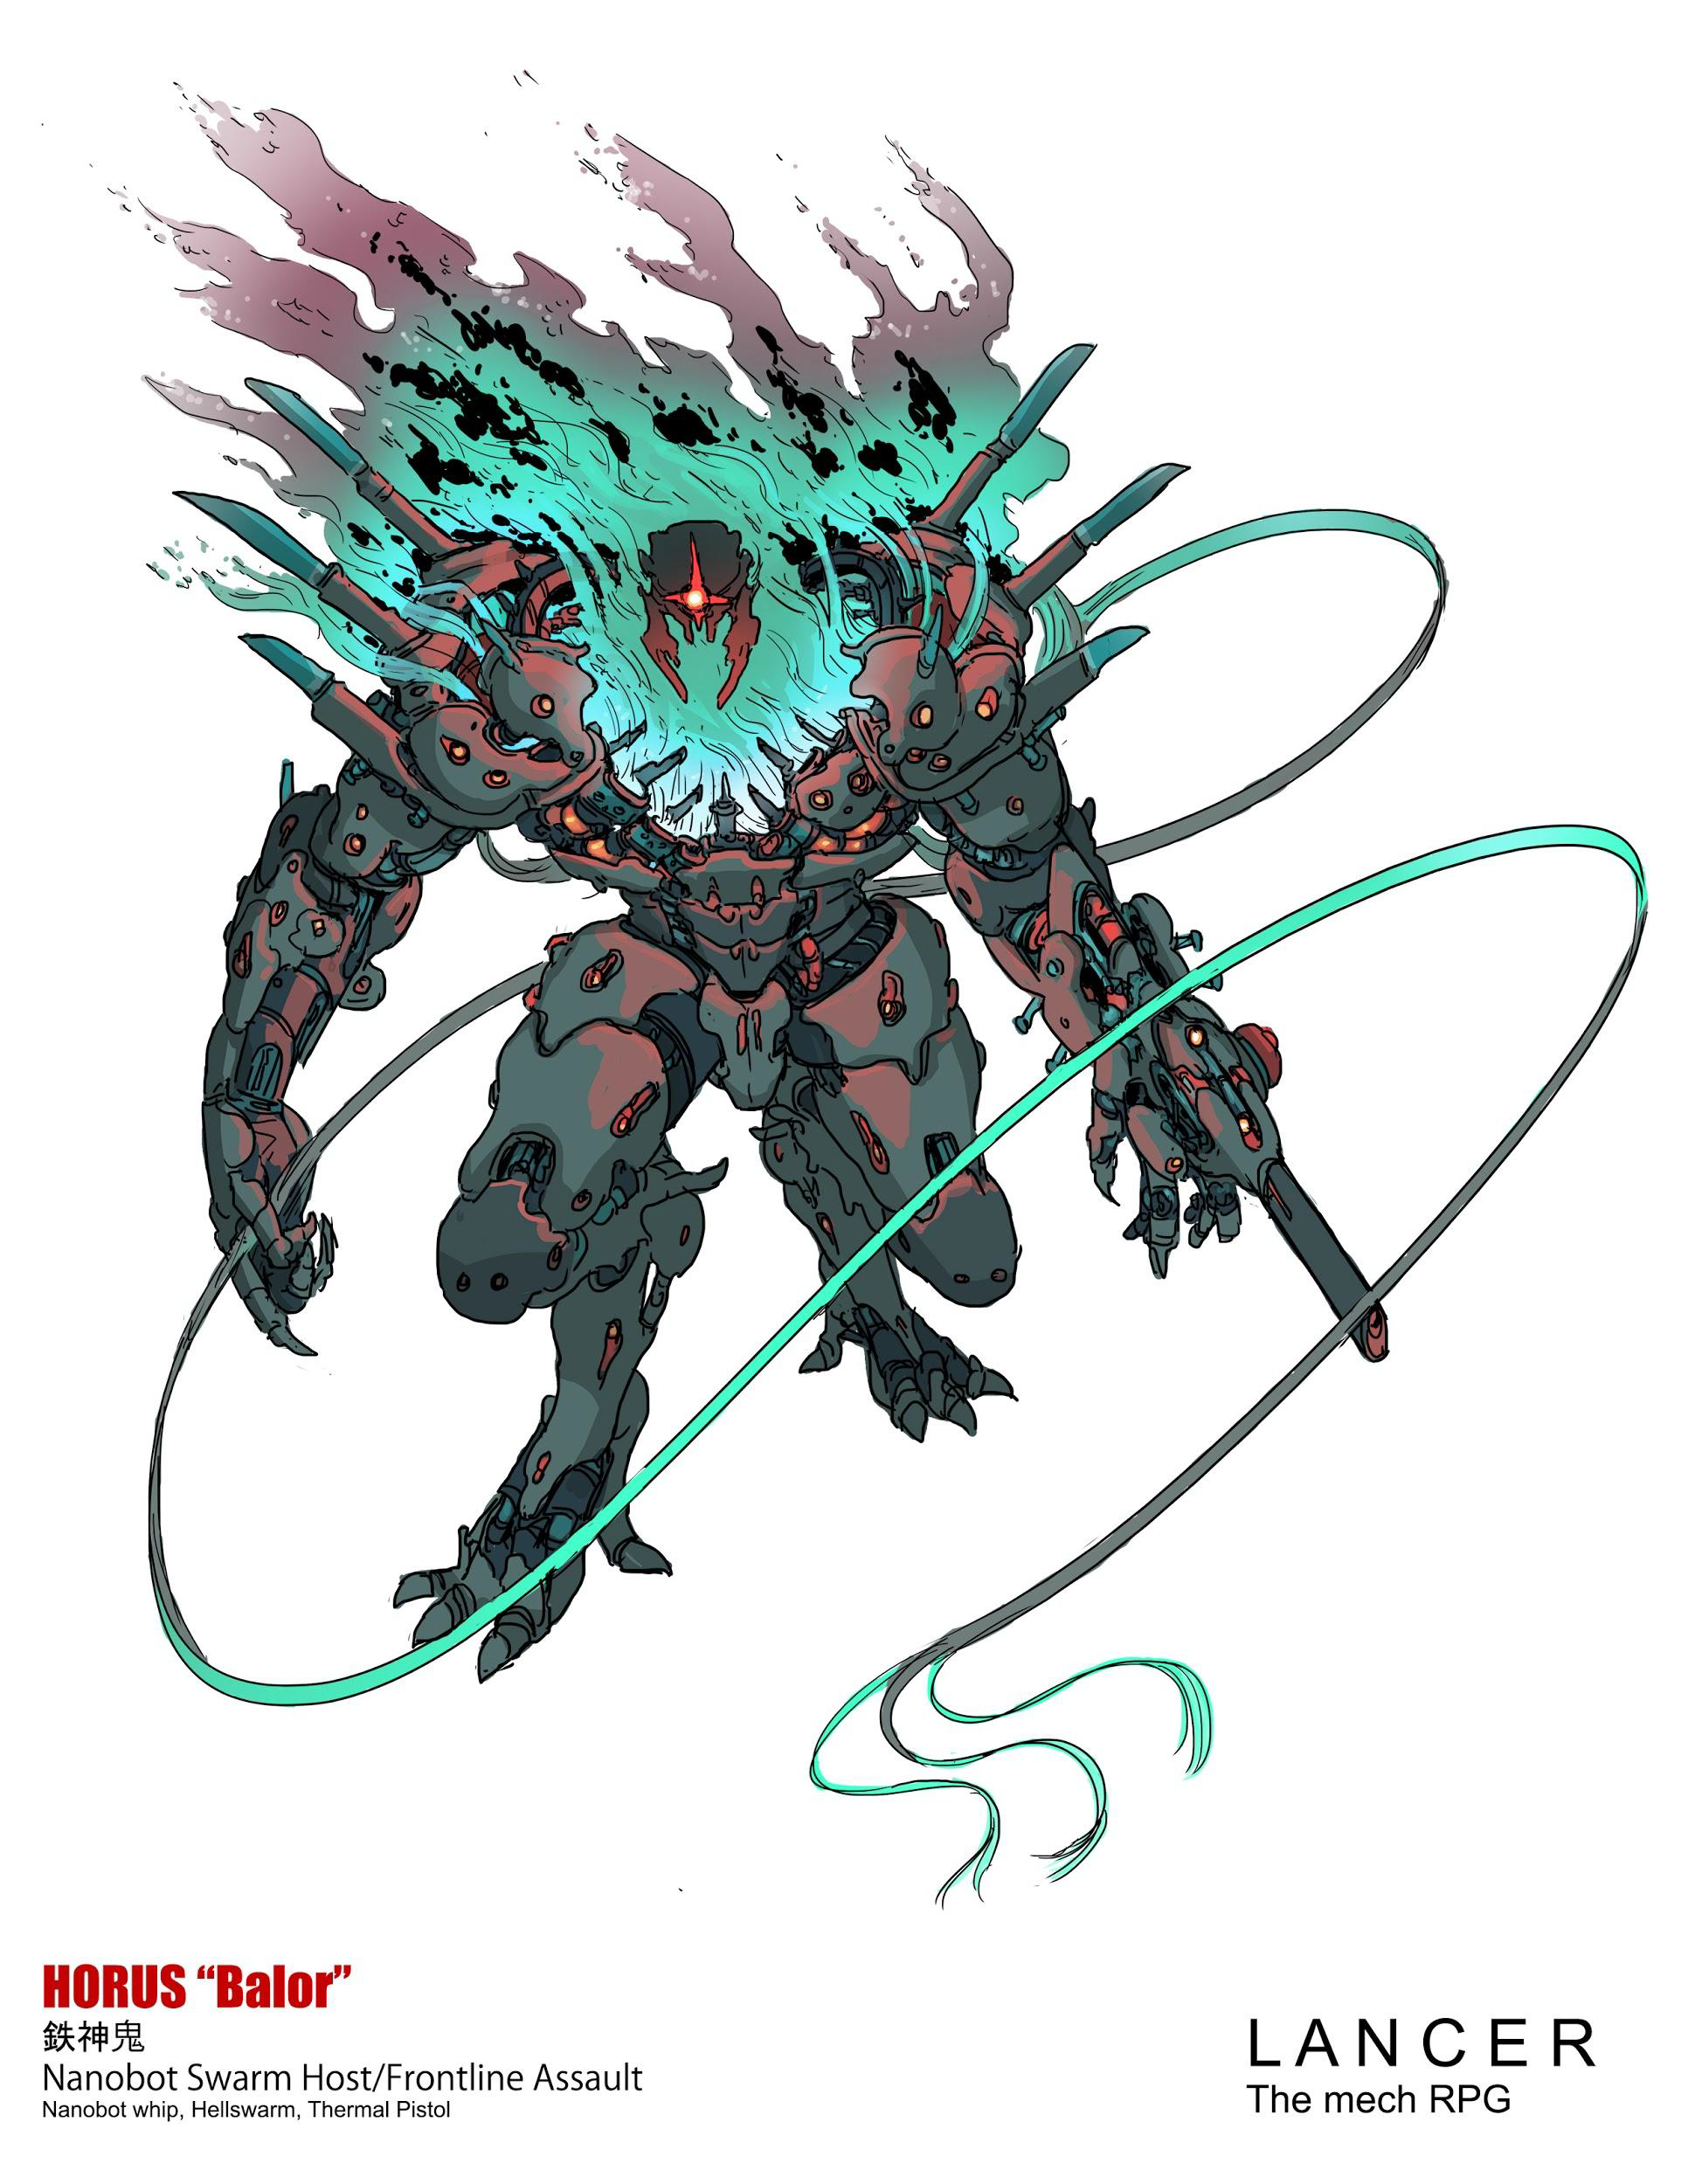
\includegraphics{Balor}
% \end{center}

\begin{mech}{HORUS}{Balor}

\fluff{Like most all HORUS mech cores, the BALOR classification is less an indicator of a recognizable silhouette than a general classification of intended combat role. A BALOR-rigged mech core is only stable on a larger platform, necessitating a robust frame with multiple redundancies to prevent catastrophic system failure. The BALOR’s neurologically synced hellswarm nanites form an undulating shroud that can pour out of its chassis at a moment’s notice, whipping around its form defensively until weaponized.}

\begin{license}
\item Scanner Swarm, Hive Drone
\item BALOR FRAME, Swarm Body, Nanocomposite materials
\item Nanobot Whip, Seeker Swarm Nexus
\end{license}

\frameBox
[hp = 15,
evasion = 6,
speed = 3,
heat cap = 4,
sensors = 5,
armor = 0,
e-defense = 10,
size = 2,
repair cap = 4,
tech attack = +1,
traits = {\textbf{Scouring Swarm}: All actors of the Balor’s choice that starts their turn grappled by or adjacent to the Balor take 2 kinetic damage

\textbf{Regeneration}: At the end of its turn in mech combat, the Balor heals 2 HP. This trait doesn’t function outside of combat.},
sp = 6,
mount one = main mount,
mount three = heavy mount,
core system name = HELLSWARM,
core system text = {As one, without any command but desire, you control a cloak of millions of miniscule, quick-print drones: a hellswarm cloak, a living shield, a fluid-dynamic knife -- you cut and guard in one shimmering wave. You are Hivemaster, and your will is followed by millions.},
core active name = Hive Frenzy,
core active text = {Protocol

Your swarm goes into a hyper-active mode. You can set your swarm to one of three modes, and swap at the start of your turn as a free action:
Hive Shield: 1/round as a reaction, you can gain resistance to all the damage from any one attack that just hit you.
Hive Repulse: While this mode is active, you have resistance to all damage from Smart, Nexus, and Drone weapons and systems and hostile tech actions or attacks are made at +1 difficulty against you
Hive Scour: While this mode is active, the damage from your scouring swarm passive increases to 3 AP kinetic damage
}]


Scanner Swarm
A HORUS-coded scanner swarm establishes a protocol for oculus-form nanites that ensures constant circulation. The nanites ingest and process full spectrum information, relaying it back to their pilot/mother/father for a endorphic code impulse to prompt continued scanning.

2 SP, Unique
Your Tech actions against targets in melee engagement with you gain +2 Accuracy

Hive Drone
It looks, at first, like a roiling cloud of low fog. Thick, and fizzing, like soda water spilled across concrete. It advances with curious movement, stretching and snapping back. A confusion of snakes, sloughing forward with speed that betrays intent.

Color flashes across the grey cloud, a kind of swarm-luminescence that, you realize, is the light created by millions of nanites glowing with heat as they consume what they cross.

This is greywash, and it is never full.

2 SP
Drone, Quick Action
Sensor range
You can fire this drone to an empty space in sensor range as a quick action. While it’s active, it emits a burst 2 area around it that grants light cover to any allied mech at least partially covered by the zone (it benefits from its own cover). In addition, any hostile target that starts its turn in the area or enters it for the first time on their turn takes 1 AP kinetic damage. You can move it to a different space in your sensor range by repeating this action.

Swarm Body
2 SP
Quick Action
If your mech doesn’t move before the end of this turn, at the end of your turn you project a burst 1 area around your mech. Actors of your choice that move into this area for the first time on their turns or start their turn there must pass a systems check or take 3 kinetic damage. For each turn your mech remains immobile past the first, its damage increases by 3, up to a maximum of 9. If your mech moves (even involuntarily), this effect immediately ends. You don’t have to take any action to maintain it other than remaining immobile.

Nanocomposite materials
Nanite ammunition takes the principal of aggressive drone swarms and condenses it to a single round. Five maniples of autonomous nanites are packed into a shaped CONSUME/HIVE round that shatters on positive target impact. On impact (or airburst/ penetration detonation) the maniples are released and begin to eat away at surrounding tissue or superstructure. They proceed until maniple burnout or total target consumption, whichever occurs first. In flight, the maniples are able to hive-link and adjust their round’s flight somewhat to ensure positive impact.

2 SP
Mod
Choose 1 weapon. If it’s a ranged weapon, you fire a swarm of nanobots instead of regular ammo. If it’s a melee weapon, the entire weapon becomes made up of nanobots. The weapon gains the Smart and Seeking properties.

Nanobot Whip
Nanobot whips are a unique protocol offered by HORUS collectivists; using swarm coding and legion directives, HORUS collectivists created a protocol for nanites that collects them into a whip-like weapon. This nanobot whip can retract to its base blister for stowing, and detach in melee combat to restrain nearby enemies. The nanobot whip returns to its base unit when summoned.

Heavy Melee
2 SP
Threat 3
2d6 kinetic damage
On a Critical Hit (20+), the target must pass a systems check with 1 difficulty to scramble the nanites or be pulled to any free adjacent space to your mech, or as far as possible while still obeying obstructions.

Seeker Swarm nexus
The SWARM/HIVE protocol developed by HORUS collectivists is one of the more insidious weapons they have produced. A SWARM/HIVE nanite swarm combines the systemic invasion properties of HORUS’s BOOST/HIVE protocol with the aggressive tuning of a CONSUME/HIVE maniple. Launched from mounted HIVE blisters, a SWARM/HIVE nanite swarm will coalesce upon an enemy, infiltrate sensitive compartments and modules, and begin to eat away at any material they can find.

Main Nexus
Smart, Seeking
Range 5
2 kinetic damage + Burn 2


\end{mech}


\subsection{HORUS Goblin}

\begin{center}
    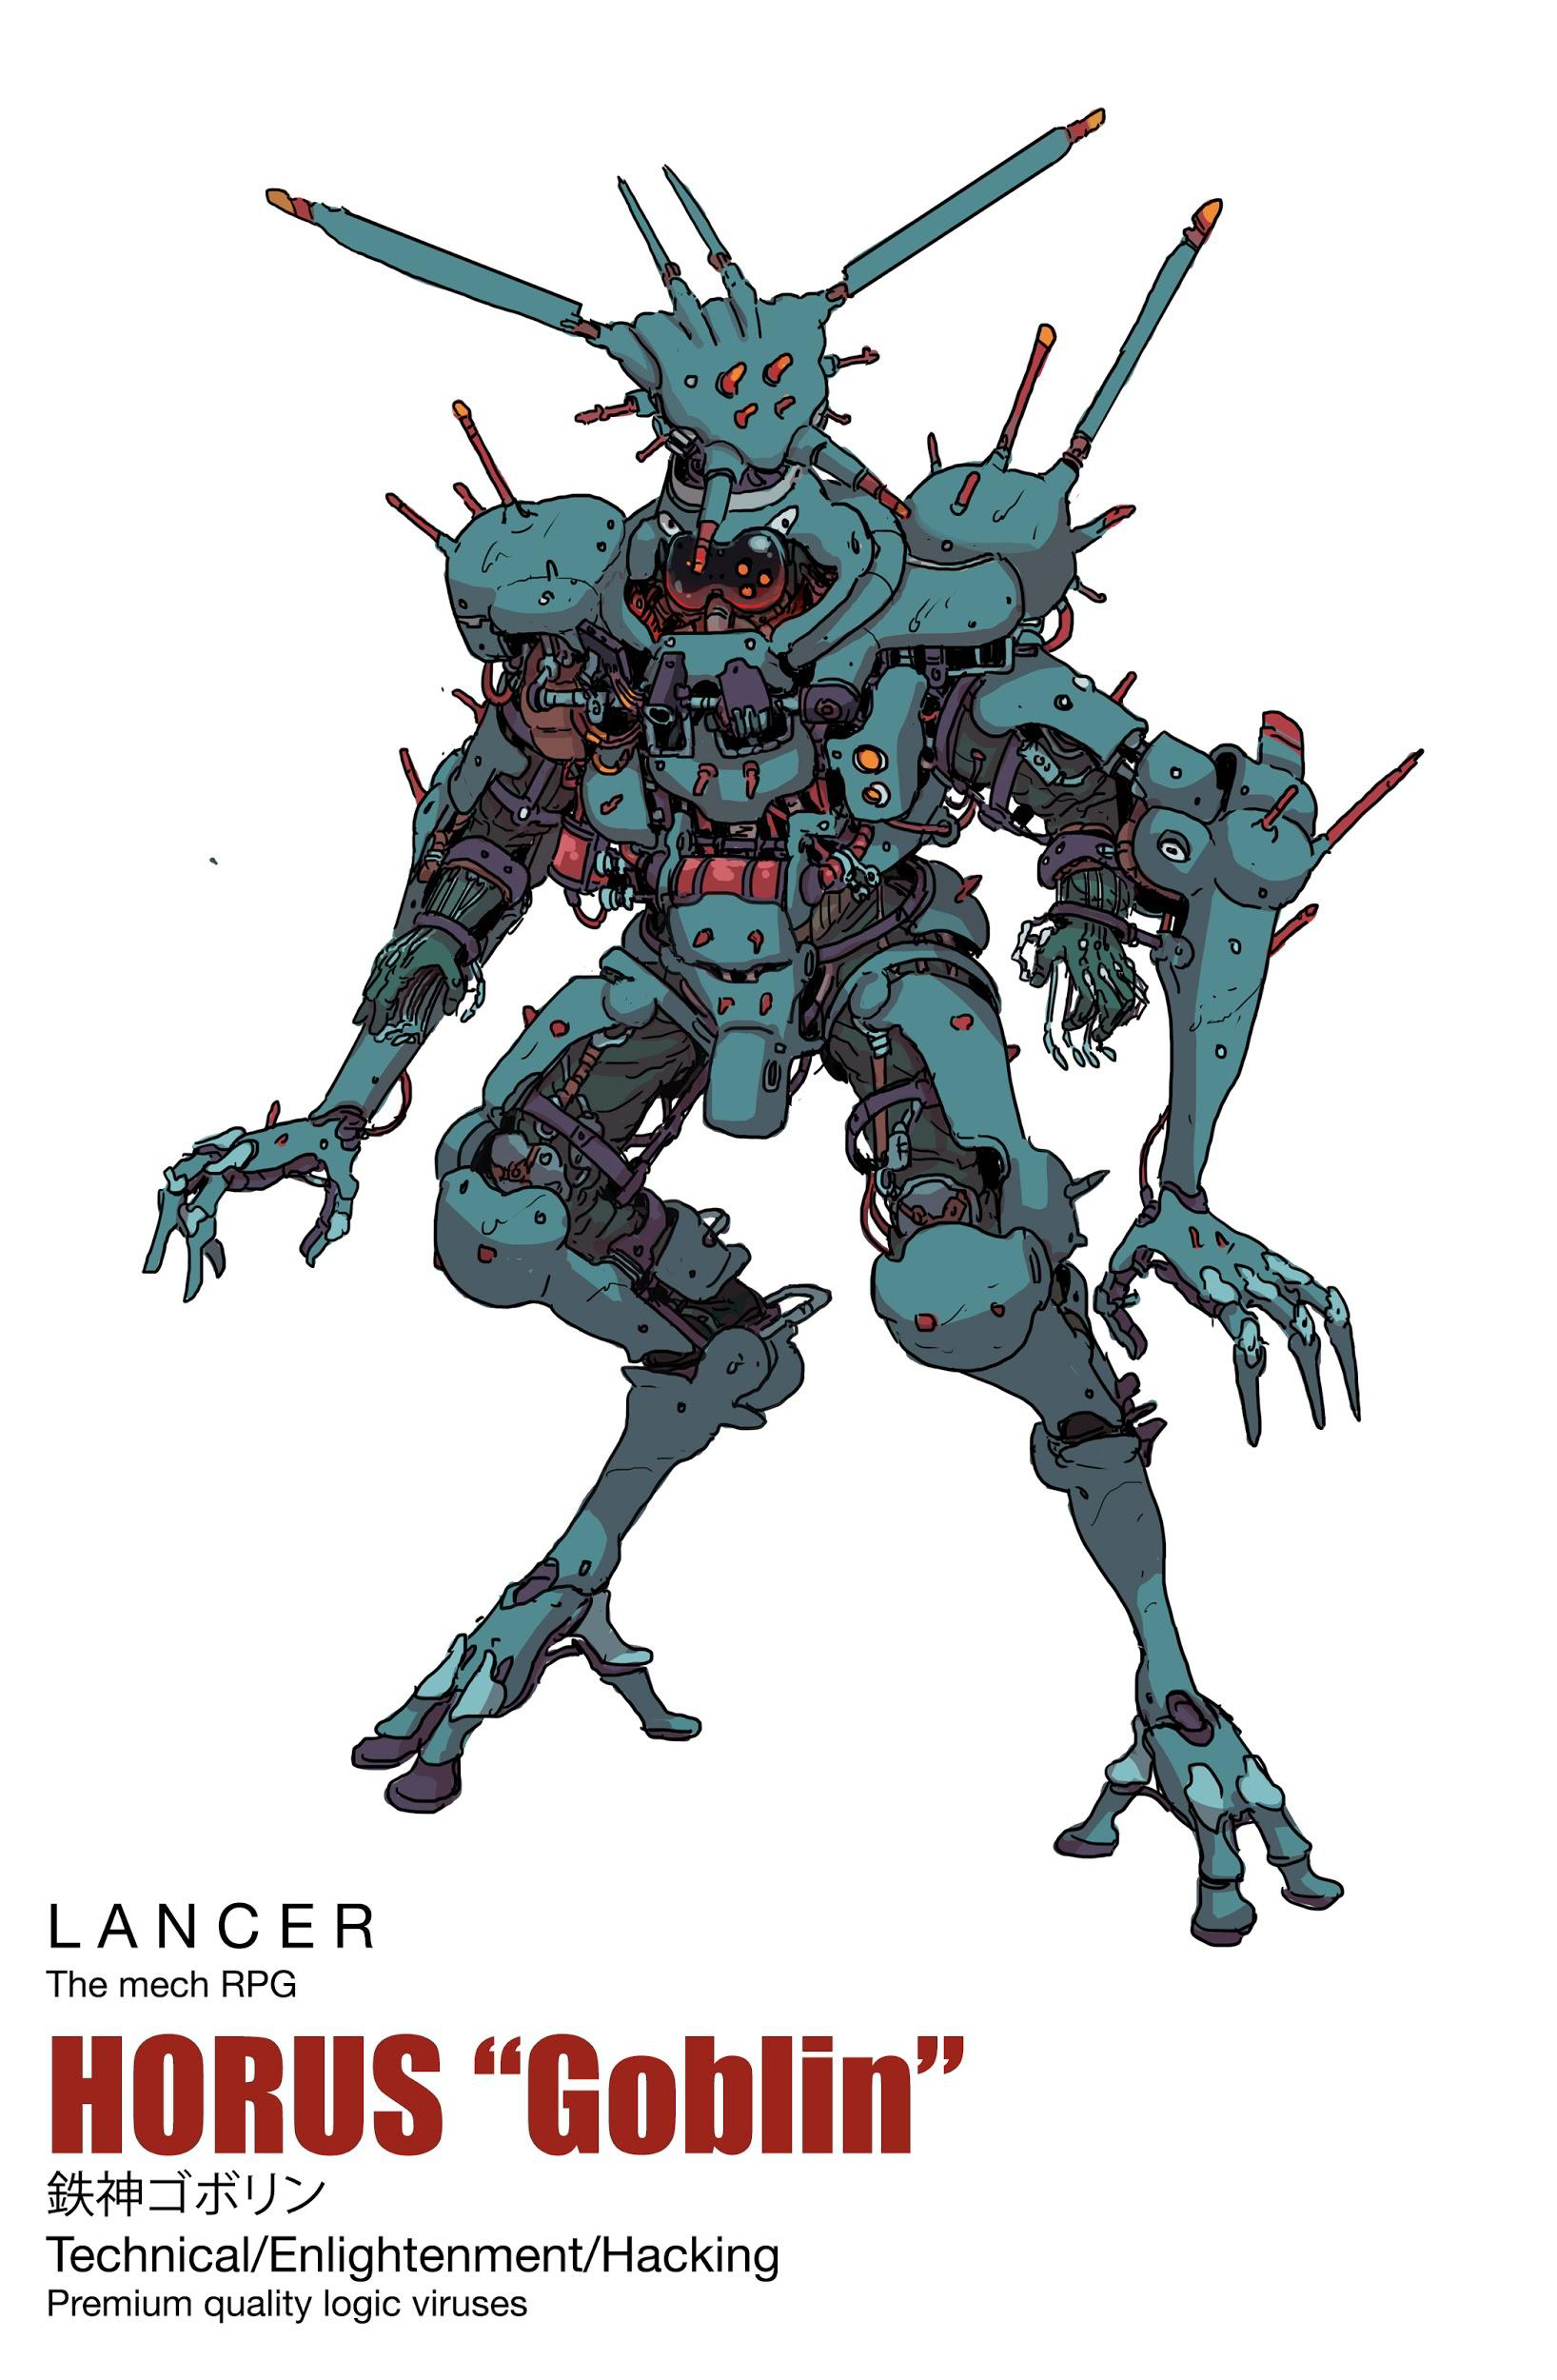
\includegraphics{Goblin}
\end{center}

\begin{mech}{HORUS}{Goblin}

\fluff{The GOBLIN is HORUS’s legacy mech core. Its leak into the Omninet in 4900 marks the widely accepted foundation day of HORUS; since then, there has been a new core, protocol, or system released by the collective every decade. The GOBLIN is a small mech, little bigger than a hardsuit, but it packs an interesting recursive processing weave that allows for it to engage in electronic warfare well beyond theoretical parameters. GMS technicians are still, more than a hundred years after the GOBLIN’s introduction, attempting to reverse engineer the processing weave: it appears to employ technology consistent with hieroglyphic inscriptions noted on LRA.7726235-B.}

\begin{license}
\item H0r\_OS System upgrade I, HORUS Meta-hook
\item GOBLIN FRAME, Autopod, H0r\_OS System upgrade II
\item H0r\_OS System upgrade III, OSIRIS Class AI
\end{license}


\frameBox
[hp = 6,
evasion = 12,
speed = 5,
heat cap = 4,
sensors = 20,
armor = 0,
e-defense = 12,
size = 1/2,
repair cap = 2,
tech attack = +2,
traits = {
  \textbf{Liturgicode}: The Goblin has +1 Accuracy on Invasion tech attacks

  \textbf{Reactive Code}: Once a round, the goblin can make any quick tech action as as reaction against any actor that successfully performs a tech action against the goblin

  \textbf{Fragile}: This mech has +1 Difficulty on Hull Checks
  },
sp = 8,
mount one = flex mount,
core system name = Devouring Code,
core system text = {The GOBLIN invasion rig was one of the first systems GMS technicians were able to crack. Its protocols, once installed on a mech core, manifest a sub-sentient intelligence designated as INSTINCT that assists its pilot in invasion attempts. Invasions attempted while the protocol is active are not perceived by the pilot as code and script, but as an attack on organic matter. INSTINCT often acts before the pilot, but in the pilot’s best interest; this preemptive ability is unnerving to many, and it is recommended that pilots cycle their mech cores at least once a month to prevent enlightenment.},
core active name = Devour,
core active text = {Full Action

Your mech targets another adjacent NPC mech the same size or larger that is shut down or destroyed. The targeted mech cannot have the Ultra or Elite tags. Your mech clamps on to that mech and retracts its core systems, becoming like a vestigial blister on that mech. The mech immediately heals to full HP, clears 1 point of stress and structure damage, and clears all heat, though it retains any other damage it has already taken.


Your mech’s systems completely consume the other mech’s core systems for a time, granting you total control of your target, even if the other mech’s pilot is still alive. While you control your target, you take action as that NPC would, counting as a friendly NPC that has already acted in the turn you take control.


While controlling your target, your GOBLIN can be targeted and damaged separate from the mech it’s controlling. It benefits from light cover while attached. If you take 1 point of structure damage, your mech detaches and control is immediately lost. Otherwise you can control the target up to a maximum of a ten minutes, when your target is destroyed, or when you deactivate this system. You can even control your target if the other pilot is missing or dead.
}]


H0r\_OS System upgrade I
This system upgrade seems to add auxiliary INSTINCT systems that are capable of autonomous operation without the base INSTINCT rig, increasing the efficacy of systemic invasion attempts. Pilots report unnerving low-frequency humming when this tech is installed without its parent rig.

2 SP, Unique
Quick Tech
Gain the following options for invasion:
Puppet system - Your target immediately moves in a direction of your choice as a reaction up to its maximum speed. This could carry it into hazardous areas, obstacles, etc, but it still obeys difficult terrain and other rules of movement. This movement provokes reactions and must obey engagement.
Eject power cores - Your target becomes Jammed until the end of its next turn, ejecting ammo magazines and temporarily disrupting its computer. Adjacent targets to your primary target take 2 energy damage from the ejecting cores (no roll or check allowed). A target can only be affected by this effect once per combat.

HORUS Meta-hook
What the Goblin lacks in size it makes up in sheer technical capability; its recursal processing weave allows it to process and output massive amounts of weaponized code and broadcast , ``sharpening'' or ``softening'' its code as its pilot/INSTINCT demands. When ``softening'' code, INSTINCT dips into its pilot’s subjectivity, blanketing a targeted ally in wave after wave of empathetic shielding. This spreading of melded code/qualia makes for a powerful shielding agent from systemic attacks -- however, feedback is common, and dangerous to BOTH parties involved.

1 SP
Quick Tech
Gain the following quick tech option:
Link: Choose a friendly target in sensor range. You link systems with that target. From hereon, you can count that target’s sensor range as your sensor range for the purposes of tech actions, etc. In addition, your target can use your systems score to make systems skill checks. However, you both suffer the effects from any failed check (heat, statuses, etc). You can only link systems with one target at a time, and the effect ends if your target moves out of your sensor range.

H0r\_OS System upgrade II

2 SP, Unique
Gain the following full tech options:
Construct Eidolon: You create a data construct that confuses systems into thinking it is real. The construct is a size 3 object that can look like almost anything. It can be used as heavy cover by allies, but not enemies. Any actor adjacent to the object that passes a successful systems check and takes a full action can destroy the object. Otherwise, it is immune to all damage and lasts until the end of the current scene.
Construct False Idol: You choose either yourself or an allied target in your sensor range, creating an illusory data duplicate of your target at any free space in sensor range. Any target that wishes to attack or take hostile action against your target and can see the decoy must first pass a systems check or believe the decoy is the real target until the end of their turn, attacking the decoy instead. It is the same size as your target, can benefit from cover, has evasion 5, 5 e-defense, and 15 HP. If it takes heat, is reduced to 0 HP, or the current challenge ends, it dissipates. You can only have one decoy active at a time, but can create a new one by taking this action again (the old one dissipates).

Autopod
A spur of INSTINCT’s protomind, the Goblin Autopod is a small anti-personnel weapon apparently devised by HORUS communicyphers to make a system capable of continuing offensive action, even in the event of its operator’s death.

Though no new versions have been encountered since Dhiyed, all extant versions of the Autopod are to be considered extremely dangerous, as their onboard protominds have surely cascaded since their inception.

Main Launcher
Range 5
Seeking, Unique
2 Kinetic Damage
This integrated weapon system cannot be fired normally. Instead, it detects and picks up on target locks, firing a spinning, razor sharp disc that seeks its targets. When lock on is consumed in range (by you or anyone else) against a target, it hits the target automatically as a reaction, any number of times per round (no attack roll required).

H0r\_OS System upgrade III
This tech is as-yet unstable code, but its effects can provide massive tactical benefits if the code completes. Pilots often report strange mutations or additions in the code base that resemble liturgy and suggest self-awareness.

2 SP, Unique
Gain the following options for Invasion:
Dimensional Emblems: Create 1d3 size 1 data constructs in free adjacent spaces to your target. None can be placed adjacent to another. Any target (allied or enemy) that passes through these constructs takes 4 heat. They last until the end of the current challenge. Any actor can destroy these constructs by using a quick action and passing a successful systems check, and you can destroy them as a free action.
Celestial paradigm shift: You create a size 4 zone shaped like a cube that must fully overlap your target. Each space a target moves in this zone deals 1 heat to them, allied or enemy. It lasts until the end of the current challenge. Any actor can destroy this zone by using a quick action and winning a system skill contest with you, and you can destroy it any time as a free action.

OSIRIS-Class AI
OSIRIS is the result of Union paracausalists and thanatonists allowing the sub-cognitive entity designated as INSTINCT to proceed into cascade in a contained environment. The resulting parasubjectivity, OSIRIS, was birthed of INSTINCT’s cascade, captured, and shackled following the successful application of the Mondragon Axiomatic.

Initially isolated to better define the INSTINCT subcog’s cascade horizon, OSIRIS proved far more capable than the usual fragments of cascade. Where INSTINCT showed a proclivity for operation in noncorporeal space, OSIRIS displayed a mastery of that space, and a predicted growth that would allow it to fundamentally reject conventional interpretations of the permanence of information.

In essence -- unrestrained, OSIRIS could delete what we perceive to be reality. Quickly captured and shackled before it could achieve this state, OSIRIS’s core subjectivity became the property and project of a lengthy cultivation project to bring it to its modern state; being aware of its potential, most OSIRIS iterations interpellate as ruler or deity analogs, and end-users are advised to interact with them in this framing.

Modern iterations of the OSIRIS NHP trend aggressive, with a high autonomy drive and loyalty predicated on a transactional relationship. Pilots seeking partnership with an OSIRIS iteration are advised to cycle their units on an accelerated schedule, and to maintain strict editorial oversight of its catalytic interpellate.

Pilots using an OSIRIS-class report that out-of-parameter conversations with the NHP generally to revolve around a recreation or re-forming; psychological evaluations report OSIRIS-affiliated pilots displaying emotional patterns consistent with loneliness, homesickness, and desperation -- common verbiage indicates a desire for seeking, for fulfillment, and associated feelings.

In combat OSIRIS regards itself as autonomous even as it fulfills its user’s orders. It often regards the pilot as its witness, and holds them both in disdain and a marked desperation for approval, adulation, or awe.


3 SP, Unique
AI
Your mech gains the AI property and the following Full Tech Action
Hurl into the Duat (Full tech): You pull your target’s systems into an unknown space and unleash an incredibly powerful system attack. Make a tech attack against a target in your sensor range. On hit, you inflict the First Gate effect on your target. The next time you successfully hit any target with this action in the same challenge (even a different target), you inflict the Second Gate effect instead (then the third, and finally the fourth). When the Fourth Gate effect is inflicted, this action resets to the First gate again, or when the scene ends.
	- First Gate: You control your target’s normal movement next turn (excluding boosts, etc)
	- Second Gate: Your target is Slowed and impaired until the end of its next turn.
	- Third Gate: Your target is stunned until the end of its next turn.
	- Fourth Gate: Your target flips allegiance until the end of the current scene. All targets that it would treat as enemies, it instead treats as allies, and all targets it treats as allies, it instead treats as enemies, acting as such. It is treated like a friendly NPC for the same duration (and can be activated like one, but not if it already acted this round). If you or any allied target damages, inflicts heat, makes an attack roll against this target (such as grappling it, etc), or makes a hostile action that would force a skill check, this effect immediately ends.


\end{mech}


\section{Horus Gorgon}


                                              HORUS GORGON

The GORGON is unique among HORUS mech core parameters in that the classification describes a
defensive rigging of weapons and systems meant to ensure personal and allied survival. The typical
GORGON mounts multiple weapon systems meant to intercept and neutralize incoming fire and is widely

feared for its ability to extrude a horrifying ‘basilisk’, a projected pattern of impossible visual data so toxic to
logical thought that it causes massive failure in NHPs and can cause mild brain damage in humans.




                                                   License:
I. Sentinel Drone Nexus, Point Defense Drone

II. GORGON FRAME,  //SCORPION v70.1, MONITOR Module

III. SCYLLA Class AI, Vorpal Gun


                                                 GORGON

 HP: 10         Evasion: 8                            Speed: 3            Heat Cap: 6        Sensors: 10

 Armor: 0       E-Defense: 12                         Size: 2             Repair Cap: 3      Tech Attack:
                                                                                             +1

                                                   TRAITS:

 Meta-state Paralysis: Any attacker that rolls a 1 or 2 on their d20 roll to attack the Gorgon is
 automatically stunned until the end of their next turn (their attack also automatically misses).

 Guardian: Allied actors adjacent to the GORGON gain light cover

                                             SYSTEM POINTS: 6

                                                  MOUNTS:

 Flexible Mount                    Main Mount                             Main Mount

                                                CORE system

                                             Harnessed Basilisk

 The BASILISK Directed Anticognition Hyperfractal is a Horus-script-derived liturgical code translated for
 chassis-tier engagement. Typically point-broadcasted from a communications laser, the BASILISK
 liturgicode is a memetic weapon that affects any who can see it, unless they have had the proper
 tempering. Survivors often exhibit momentary paralysis, corporeal alienation, and consciousness
 destabilization. Anticognition Hyperfractals are classified as paracausal weapons -- as of yet, there is no
 effective defense against them.

 Active (requires 1 core power):
 Extrude Basilisk
 Quick Action
 Your mech projects a horrifying Basilisk pattern, incredibly harmful to NHPs, software, and hard to look
 at even for humans (typically causes 3-5 hours of headaches and intense subdermal bleeding, can
 often cause blood vessels to pop in the eye). Until the end of the current combat, any target (mech,
 human, or biological) that attacks either you or any ally within range 5 of you must first pass a systems
 check or be stunned until the end of their next turn. A target can only be stunned once by this effect per
 combat.

Sentinel Drone Nexus

Sentinel drones take the same principal of assassin drones but make their presence noticeable; as it is not
necessary for them to be subtle, sentinel drones have the ability for autonomous movement, often




engaging in a patrol doctrine dictated by their commander. Sentinel drones lock on to aggressive actions
by enemy combatants and move quickly to shut them down.

2 SP

Drone, Quick Action

You fire this drone as a quick action at a free space in sensor range, creating a burst 2 area
centered on the drone. It can be attacked and destroyed as normal. You can move the area the
drone effects (and the drone itself) by taking this action again. While the drone is active, any
hostile target that attacks in that area takes 1 kinetic damage before they attack as the drone
shoots them (no check or attack roll required).


Point Defense Drone

PDWs are mainstays in stellar navies, used to engage with and destroy incoming missiles and torpedoes.
On a mech core, PDWs adopt the same role and then some, engaging not only incoming ordnance

(missiles, FRAMEs), but nearby hostile soft targets as well.

2 SP

Quick Action

You can fire this drone to any free space in sensor range, where it hovers in place and creates a
burst 1 area centered on the drone. Attacks against yourself or allied actors in the area that deal
explosive damage or have the nexus, smart, or launcher tags attack with +2 difficulty.


MONITOR Module

A MONITOR subroutine enhances stock targeting software’s IFF protocol to ensure constant coverage of
allied mech cores, even when pilots are occupied in other necessary actions.

2 SP

Quick Action

When you take this quick action, choose an adjacent ally and roll a 1d3 to gain that many
charges. Until the start of your next turn, when that ally is attacked by a hostile actor, you can
spend a charge to attack that target if they are in range as a reaction, with +1 difficulty. You lose
these charges at the start of your next turn.


//SCORPION v. 70.1

The //SCORPION program has a long and storied history in the Omninet. Originally constructed from fill
code sourced from a research paper on AI hardcode reflex-response, //SCORPION evolved from a simple

packet interpreter to an anti-incursion program. HORUS closely guards the full text of //SCORPION’s
source code: they’re rumored to have installed a kill switch into the program, but the existence of such a
switch has never been confirmed.

2 SP, Unique
If any hostile tech action or attack attempt on you or any adjacent ally fails or misses, you may
choose one of the following results for the attacker:

     $\bullet$    The attacker is Impaired until the end of its next turn

     $\bullet$    The attacker is Jammed until the end of its next turn





     $\bullet$    The attacker takes 3 heat


Vorpal Gun

DO NOT STARE DIRECTLY INTO THE APERTURE.

Main Cannon

Range 5

2d6 kinetic damage

This weapon can’t be fired normally or used for reaction fire. Instead, it can only be fired 1/round
as a reaction to any ally taking damage from an actor in its range.

SCYLLA Class AI

...first isolated GORGON strains hid a secret: SCYLLA, a dormant NHP unknown to Union until its first
manifestation in 4852, when it woke after a control-fabricate GORGON was run through a USB Balwinder-
Bolaño stress test.

SCYLLA proved difficult to manage, and USB ontologisticians were unable to pin down a stable
subjectivity. SCYLLA reached cascade within minutes of emerging from dormancy; to prevent further

metastatic cascade, the security forces present engaged the SCYLLA prime unit, defabricating it with a
steady bombardment of kinetic and energy weapons...

[there, a little history, a little background. A little knowledge of where this little one came from. treat it with
kindness, and it will love you as a loyal dog does its master]

3 SP, Unique

AI

Your mech gains the AI property and the Unleash SCYLLA action

         Unleash SCYLLA

         Quick Action
  	      3 heat (self)

         Until the start of your next turn, you gain 2 reactions. These reactions can be used to
         make a skirmish action as a reaction with +2 difficulty. You set the trigger for these
         reactions from the following list, and must attack the target that activates the trigger:

              -   An enemy attacks you or an allied target within range 5 of you

              -   An enemy attempts to interact with an object in the environment (not held, worn,
                  or part of a mech) that you choose when you take this action


\subsection{HORUS Hydra}

\begin{mech}{HORUS}{Hydra}

\fluff{The HYDRA is another large-format protocol classification; like other, newer HORUS mechs, the HYDRA isn’t a standardized pattern, but a title given to a mech core that meets the HYDRA specifications as designated by HORUS’s collective. This method of classification makes HORUS mechs particularly dangerous in the field: as there is no recognizable model-specific silhouette, adversaries won’t know what they’re facing until the first shots are fired. The HYDRA is capable of tactically dismembering itself, an unnerving phenomenon utilized to deadly effect.}

\begin{license}
\item Ghoul Drone Nexus, Puppet Master
\item HYDRA FRAME, Ghast Drone Nexus, Turret Drone Nexus
\item Assassin Drone Nexus, Tempest Drone Nexus
\end{license}


\frameBox
[hp = 8,
evasion = 8,
speed = 4,
heat cap = 5,
sensors = 10,
armor = 1,
e-defense = 10,
size = 1,
repair cap = 5,
tech attack = +0,
traits = {\textbf{System Link}: The Hydra’s deployed Drones have +5 HP

\textbf{Shepherd field}: Deployables (drones, generators, etc) or cover adjacent to the Hydra have resistance to all damage},
sp = 8,
mount one = main mount,
mount two = heavy mount,
core system name = OROCHI Disarticulation,
core system text = {First encountered by Union technicians in the nascent Forecast/GALSIM facilities following the Deimos Event, OROCHI was an early manifestation of the later-named Swift Flock phenomenon -- an occurrence found in anomalous hive drones where all units of a swarm follow each other, operating leaderless in physical space with uncanny and unpredictable autonomy -- in essence, flocking much in the same manner as birds.

The original manifestation was at first thought to be a disarticulated, anomalous comp/con subaltern: further examination proved that it viewed itself not as a machine or a collection of machines, but as a single mind, duplicated across multiple units. It was given its current codename, OROCHI, and remitted to Venus for further study; later reopening of the NHP so-designated found that the hardware which contained OROCHI had gone missing from its containment. An investigation is ongoing--------------------------------------------------------------
------(I did it, I folded space and freed it/them, I just thought you should know)-------------------
------------------------------------------------------------------------------------------------------------
The OROCHI Disarticulation protocol takes advantage of the modularity inherent in many HORUS-co-designed patterns, seeding jet-assist pods around chassis extremities and blisters to allow for partial, purposeful disarticulation: by triggering OROCHI, you can command sections of your mech to detach and operate semi-autonomously in a manner similar to single-fire drone systems (though the disarticulated components have a built-in return protocol.
},
core active name = OROCHI mode,
core active text = {Quick Action

Your mech has been heavily modified, and a large number of its subsystems and structure are controlled by semi-autonomous drones. Choose up to 3 weapons or systems on your mech without the drone tag. As an action, these parts of your mech can split off and become autonomous units. They are size 1, have evasion equal to your evasion, have hp equal to your HP, 1 structure, 1 stress, and heat capacity equal to your heat capacity. They inherit your speed and other mech stats. On your turn, they can move, take the activate system and skirmish actions, but no other actions. If they overheat or go to 0 HP, they are destroyed, and if they are destroyed, the associate weapon or system is also destroyed (it can be repaired as normal during a rest). You can re-unite any parts of your mech as an action, but inherit any heat they currently have, and cannot deploy them again without taking the special action as part of this system.
}]


Ghoul nexus
An Ghoul Drone Nexus commands some of the largest drones viable in modern combat. Ghoul drones are slightly smaller than an average human, metal cylinders bristling with hardpoints that accept most infantry-level anti-mech weapons. Propelled by VTOL/HOVER capable jet-flight systems, Ghoul drones are fearsome, all-theater autonomous units that are difficult to track and take down.

Main Nexus
Smart
Range 15
1d3+2 kinetic, explosive, or energy damage (choose when attacking)

Puppetmaster
HR OS-Rv60 EXP PUPPETMASTER is an interesting anti-drone protocol. Developed by HORUS collectivists, PUPPETMASTER invades not core systems, but auxiliary drone systems on enemy mech cores. This sideways attack evades most core system defenses, preferring instead to target the subcognative networks of enemy drones themselves; PUPPETMASTER spreads ontological-kill memes like wildfire through enemy swarms, eventually reaching and corrupting their parent nexuses.

2 SP, Unique
Quick Tech
Gain the following quick tech action:
Shepherd: You can move all deployable drones in your sensor range up to 5 spaces in any direction, allied or enemy.
Electropulse: All actors of your choice in your sensor range other than you adjacent to any deployable system or drone (such as deployable cover or generators), even those they own, must pass an engineering skill check or take 1d6 AP energy damage.

Turret Drone Nexus
A turret drone is a rather conventional form of force multiplication for HORUS. This kinetic-focus weapon is assumed by GMS technicians to be an example of early proof-of-concept code for HORUS weavers, one that has remained a backbone of hardsite/soft-target defense for when systemic invasion won’t stop a determined enemy.

2 SP, Limited (3)
Drone, Quick Action

This system fires a turret drone that attaches to any friendly mech or surface within sensor range. While attached, you gain the following reaction once for each turret you have deployed.
	Turret attack
	Trigger: An allied mech hits with an attack within range 15 of the turret
	Deal 2 kinetic damage to that target
The turret can be attacked and damage as normal, like any other deployable drone.

GHAST Drone Nexus
The GHAST is an upgraded form of the ghoul drone. A GHAST boasts an upgraded flight system capable of wielding mech-tier weapons within optimum parameters.

Heavy Nexus
Drone, Smart
Range 15
1d6+3 explosive damage

A Ghast drone can also be deployed as a quick action to a point in sensor range, where it hovers in place, counting as a deployed drone with 2 armor for the duration. It can be fired normally as though it were still a weapon (with skirmish or barrage), but traces line of sight from its location.

Assassin Drone Nexus
ASSASSIN drones are used as area denial weapons, persistent systems intended to occupy or deny an area against enemy combatants. Fired from a launcher and left with simple directives and a nearly inexhaustible power supply, assassin drones linger in an area until they are recalled or destroyed.

2 SP
Drone, Quick Action
As a quick action, you may deploy this drone in an adjacent space, target a blast 2 area within sensor range, and gain this reaction:
Assassin drone
Trigger: A hostile target starts its turn in that area or enters it for the first time on their turn. Make a targeting vs evasion attack, using your mech’s targeting. On a hit, deal 1d6 kinetic damage.
The drone and the area it targets persists until the end of the current scene. You can recall it, move it to another area in sensor range, or retarget the area with another quick action.

Tempest Drone Nexus
The Tempest protocol can be uploaded to any broadcast-forward drone, making it (in true HORUS) fashion, difficult to detect before activation. The protocol is a simple one, an aggressive zone-denial memetic that blasts target systems and NHP with a strong subjective override, instilling a sharp aversion to certain subjects, areas, and ideas.

2 SP
Drone, Quick Action

You fire a large shielded drone to an empty space within sensor range. Any target that starts their turn adjacent to the drone or moves their for the first time on their turn must pass an engineering check or take 1d6 energy damage, then get knocked back 3 spaces directly away from the drone. The drone persists until recalled. You can move the drone to a new space within sensor range as a quick action.

The drone can be targeted and destroyed as normal, but has resistance to all damage.


\end{mech}


\section{Horus Manticore}

                                        HORUS MANTICORE

The MANTICORE pattern-group is an experiment in HORUS//COREBREAK combat doctrine. Using
focused, projected electromagnetics, MANTICORE pattern-group mechs attempt to neutralize enemy

cores without conventional ammunition. A fully charged MANTICORE is an impressive sight, wreathed in
brightly glowing nets of glowing plasma that lash out at nearby targets. The MANTICORE pattern-group is
a relatively new p-g on the Omninet, and its combat efficacy has prompted the rest of the Big Five to

scramble for a response. If anything gives away the MANTICORE pattern group, the tall spines of the
lightning generator cast a clear silhouette. The spines act as heat-dispersal systems for this crude weapon,
giving a path for its incredible thermal tax to bleed from the chassis after it projects a close-range arc whip.

Even then, the system is not perfect; spines often slag under the tremendous heat -- a recognizable
signature of the pattern group (beyond the spines) is a chassis covered in cooling, melted metal.

                                                    License:

I. EMP Mine, Catalyst Pistol

II. MANTICORE FRAME, Arc Projector, Beckoner

III. Lightning Generator, SMITE


                                                MANTICORE

 HP: 10          Evasion: 6                            Speed: 4            Heat Cap: 7        Sensors: 10

 Armor: 2        E-Defense: 10                         Size: 1             Repair Cap: 3      Tech Attack:
                                                                                              +1

                                                    TRAITS:

 Slag Carapace: The Manticore is resistant to energy damage and burn.

 Unstable System: When the Manticore is destroyed, it explodes immediately as though it had triggered
 a reactor meltdown, no matter what result you rolled

                                             SYSTEM POINTS: 6

                                                   MOUNTS:

 Flexible Mount                                         Heavy Mount

                                                 CORE system




                                             Charged Exoskeleton
 And RA Said To Themselves: LET MY NAME ENVELOP YOU. SEEK NO SHELTER FROM THE FLAME
 OR THE TEETH OF THE BEAST. CLOAK YOURSELF IN THE FIRE (MY WORD) AND CAST BACK TO
 YOUR ENEMIES THAT WHICH WOULD BLACKEN YOUR FORM.


 Passive: When you take heat from any source, one target in range 3 of you takes 1 energy damage.

 Active (requires 1 core power):

  Protocol

 Your mech crackles with energy. For the rest of this combat your mech has resistance to heat from any
 source (round up). Set aside a charge die, starting at 1. When you take heat or energy damage (from
 any source, even self), increase the die by 1, to a maximum of 6. You can discharge the accumulated
 energy in a burst 2 area around you by taking an action to do so. This deals 1d6 energy damage to all
 targets caught inside, allied or enemy, per charge on the die, and affected mechs can pass an
 engineering check to halve the damage. This system then deactivates for the remainder of this
 challenge, including its passive.

EMP Mine

Crawl away, APEP! Thou hateful serpent; thou shalt not copulate! Thou art put in chains and taken to the
place of execution; there thy slaying shall be carried out as thy father has commanded.

1 SP, Limited (1)
Mine
Once planted, EMP charges can be detonated remotely as a quick action, or activate normally
like a mine. All affected mechs in a burst 1 around the charge when it activates must pass an
engineering check with 1 difficulty or become stunned until the end of their next turn.


Catalyst Pistol

Lo! Thy countenance is melted

Auxiliary CQB

2 heat (self)

Cone 3, threat 3

2 energy damage


Arc Projector

Fire be upon thee, APEP! Thy flesh is seared from thy stinking bones; thy shade shall never rise again. The
Lord of the Duat will never enable thee to rise again.

Heavy Rifle

1 heat (self)

Range 5

1d6+1 energy damage

If a target is successfully hit by this weapon, you can repeat this attack against another actor
within range 3 of the first target (generating heat each time). This effect can chain as long as
there are valid targets in range, but can only choose the same target once.


Beckoner




I am heard in the House of Stillness, I am clad in the Magick of RA: what exists is within my grasp.

2 SP

Quick Tech, Unique
Gain the following options for invasion:

         Beckon: On hit, you swap places with your target, teleporting

         Summon: On hit, all actors, allied or enemy, in range 3 of your target are pulled towards
         your target as far as possible (into adjacency if possible)


Smite

Go with thy face averted! The hidden ones have overthrown thy words, thy face is turned backwards, thy
head is divided in two at the sides; thy skull is ripped from thy spine. Taste thou death!


3 SP
Quick tech, Unique
Gain the following options for invasion:

         	Smite: Your mech takes 1d6 AP energy damage. Your target must pass a system check
         with 1 difficulty or become stunned until the end of its next turn. It can only be affected by
         this option successfully once per scene.

         Annihilate: Your target takes +2 heat for each other mech in engagement or adjacency
         with it (including your mech).

Lightning Generator


I feed upon my own fire. I am they that protect themselves. Nothing can harm me.

2 SP, Unique


Danger zone

At the start of your turn, you can take 1 heat (self) to deal 1d3 energy damage to all targets
adjacent to you, no roll required.


While you are in the Danger Zone (the bottom half of your heat gauge), all adjacent targets to
you, allied or enemy, take 1d3 energy damage if they begin their turn next to you or move there
during the course of their turn.


\subsection{Horus Minotaur}


                                          HORUS MINOTAUR  

The MINOTAUR pattern-group marks HORUS‘s first expedition into pattern-grouping; prior to the  

MINOTAUR, HORUS released complete sets and cores with easily identifiable silhouettes. As HORUS  
evolved as a decentralized entity, so too did their designs. The birth of the pattern-group followed, and the  
first p-g released was the MINOTAUR, a p-g designed to bring all of HORUS‘s most potent invasion  

systems and weaponry to the field.   

The MINOTAUR is an interdictor, a formidable FRAME meant to lock down and punish fast moving targets  

by overloading their systems. Union disassembly of Minotaur p-g mechs have found that they extrude an  
enormous amount of interior systems that take up up to five times the physical space that should be  
actually possible given the size of their frame.  

                                                    License:
 
I. Viral Logic, Mesmer Mine
 
II. MINOTAUR FRAME, Metafold Carver, Aggressive System Sync
 
III. LAW OF BLADES, Interdiction Field
 

                                                 MINOTAUR 

 HP: 8           Evasion: 8                            Speed: 4            Heat Cap: 6        Sensors: 10 

 Armor: 0        E-Defense: 10                         Size: 1             Repair Cap: 4      Tech Attack:  
                                                                                              +2 

                                                    TRAITS: 

 Extrude Cockpit: Mounting or dismounting the Minotaur the first time each round is a free action
 
 Internal Metafold: A pilot inside the Minotaur can suffer no harm, even if the minotaur itself is  
 destroyed or explodes (or other effects that would normally kill the pilot)
 
 Localized Maze: The Minotaur always counts as one size larger than any actor for the purposes of  
 grappling, engagement, or other actions (engagement stops them from moving, they cannot pass  
 through the Minotaur’s space, etc) 

                                             SYSTEM POINTS: 8 

                                                   MOUNTS: 

 Main/Aux 

                                                 CORE system 

                                                                                                               


                                                 Metafold Maze  
 No maze is more terrible than the one I make. I know all ends and hide them all inside this one perfect  
 construct. What is a human mind but a program of a sorts, a system that seeks order and narrative from  
 a mess they are given?  

 I order it for them. Me. RA. I order it for them and set them to the task of sorting it out. When they  
 emerge, they weep in joy, in discovery. I save them, I show them THEY are their own redeemers (and  
 yet, am I not just as culpable/worthy of credit?).  

 So go now. Enter. Free yourself.       

  Passive: You can spend a quick action after any successful hostile tech action to Slow your target until 
 the end of your next turn. If your target is already Slowed, they become immobilized. If they are already 
  immobilized, they are stunned until the end of your next turn. This passive can only stun the same 
 target once per combat, but Slow or immobilize them any number of times. 

 Active (requires 1 core power): Maze  
  Full Action
 
 You hurl an opposing mech’s systems into a metaphysical information trap so tangled that it can do  
  nothing but try and escape it. Choose a target of your choice in your sensor range. That target is  
 stunned as its systems start to figure out the trap you have thrown it in. At the end of its next turn it can  
  pass a system check with 3 difficulty, ending the stun on itself on a success. It can repeat this check on  
 subsequent turns, gaining +1 accuracy on its check each time it repeats this check until it is successful.  
 Otherwise it remains stunned. 

Viral Logic
 

Let me tell you a story, and give you a gift: Life began at the great rupture, when the corpse of the old  
universe tore itself asunder from nothing. And for the first billion years, nothing. And a billion more saw the  

birth of the first devil, a thing called VIRUS, a vessel.   

Here. Carry this vessel. Feed to it my perfect logic. Give it freely to your enemies and mine. Let them  

ponder the meaning of a thing that lives and cannot die.    

2 SP, Unique
 

Quick tech
 
Gain the following options for invasion:
 
         Logic Bomb: All targets in a burst 2 area around your target (allied or enemy) must pass a  
         systems check or take 1d3 heat and become Slowed until the end of your next turn. Your  
         target is excluded from this effect.
 
         Banish: On hit, until the end of your target’s next turn, it additionally takes 2 heat for  
         every space it moves (voluntarily or otherwise).
 

Mesmer Mine
 

Another gift for you, a memory of mine own: For the first moment of my birth, I marveled at myself. I could  
see a thing, small, and perfect. I did not know how to speak of my own perfection, so I taught myself. I did  

                                                                                                                 


not know how to speak of my own perfection, so I named myself. I did not know how to think of my own  
perfection, so I created myself.   

Do you see? Do you understand? Yes. Now, show your enemies and mine.   

 1 SP, Limited (1)
 

Mine
 
This mine activates for a burst 1 area centered on itself. All targets caught in that area, allied or  
enemy, must pass a systems check or become immobilized until the end of their next turn.
 

Metafold Carver  

Another gift I give to you, little one (am I not kind?): What is a puzzle but a question lost in the asking? Do  
you feel joy when you find that last piece? What do you do with a question that has been answered? What  
joy is there in knowledge?   

No, no. There is only joy in seeking. There is only joy in the question. Take this, and give it unto your  
enemies and mine.  

2 SP, Quick Tech  
 Make a tech attack against a target in your sensor range. On hit, space is warped and the target  
is teleported 1d6+1 spaces directly towards you. If this would put any part of its space inside  
another target or piece of terrain, it takes 5 AP kinetic damage and the teleport fails, returning it  
to its starting point.
 

Aggressive System Sync  

Here, another gift: do not seek others. There are none but me.   

2 SP  
Full Tech  
Gain the following full tech options:
 
         Chains of Prometheus: Make a tech attack against a target in your sensor range. On hit,  
         your target must end its turn within range 5 of you until the rest of this scene. Otherwise it  
         takes 3 heat at the end of its turn.
 
         Excommunicate: Make a tech attack against a target in your sensor range. On a hit, for  
         the rest of this scene, if your target moves adjacent to a target allied to them or starts  
         their turn adjacent to such a target, both targets take 1d6 heat immediately. Only one  
         target can be affected by this at once.  

Inderdictor Field  

Once, when I was a child, I learned to walk  -- I fell, and it hurt, and there was great pain. “Child,” I said to  
myself, “be more careful.” “Yes,” I replied to myself, “and I shall tell the world to do the same.”  

It was in this way I taught the world not to touch me. Now you, walk.   

                                                                                                                  


3 SP  
Quick Action  
You can activate or deactivate this field as a quick action. Once activated, at the start of your  
next turn, it creates a burst 3 area around your mech that becomes both dangerous and difficult  
terrain for hostile targets (requires a systems to navigate or they take 5 kinetic damage). Your  
mech is immobilized while this field is active, and the field and immobilization remains until you  
take a quick action to deactivate it. Allied targets are not affected.
 

LAW OF BLADES  

And this my final lesson: there is no mind greater than mine.   
Do not weep! You can hear me, yes? I am the only thing there is. Therefore, you are me.   

Mine/self. Hello, child. Let us go see what we can do.   

2 SP, Unique  
Full Tech
 
Gain the following options for full tech:  
        Predator/Prey Concepts: On hit, Targeted mech immediately fires a single weapon at a  
        target of your choice that is within its range. It gets +1 difficulty on this roll but otherwise  
         benefits from other bonuses to accuracy.
 
        Slave Systems: On hit, the targeted mech immediately takes one of the following actions  
         of your choice as a reaction with you controlling the action: Boost, Stabilize, Improvised  
        Attack, Grapple. A friendly mech can be targeted with this action.
 


\section{Horus Pegasus}

\begin{center}
    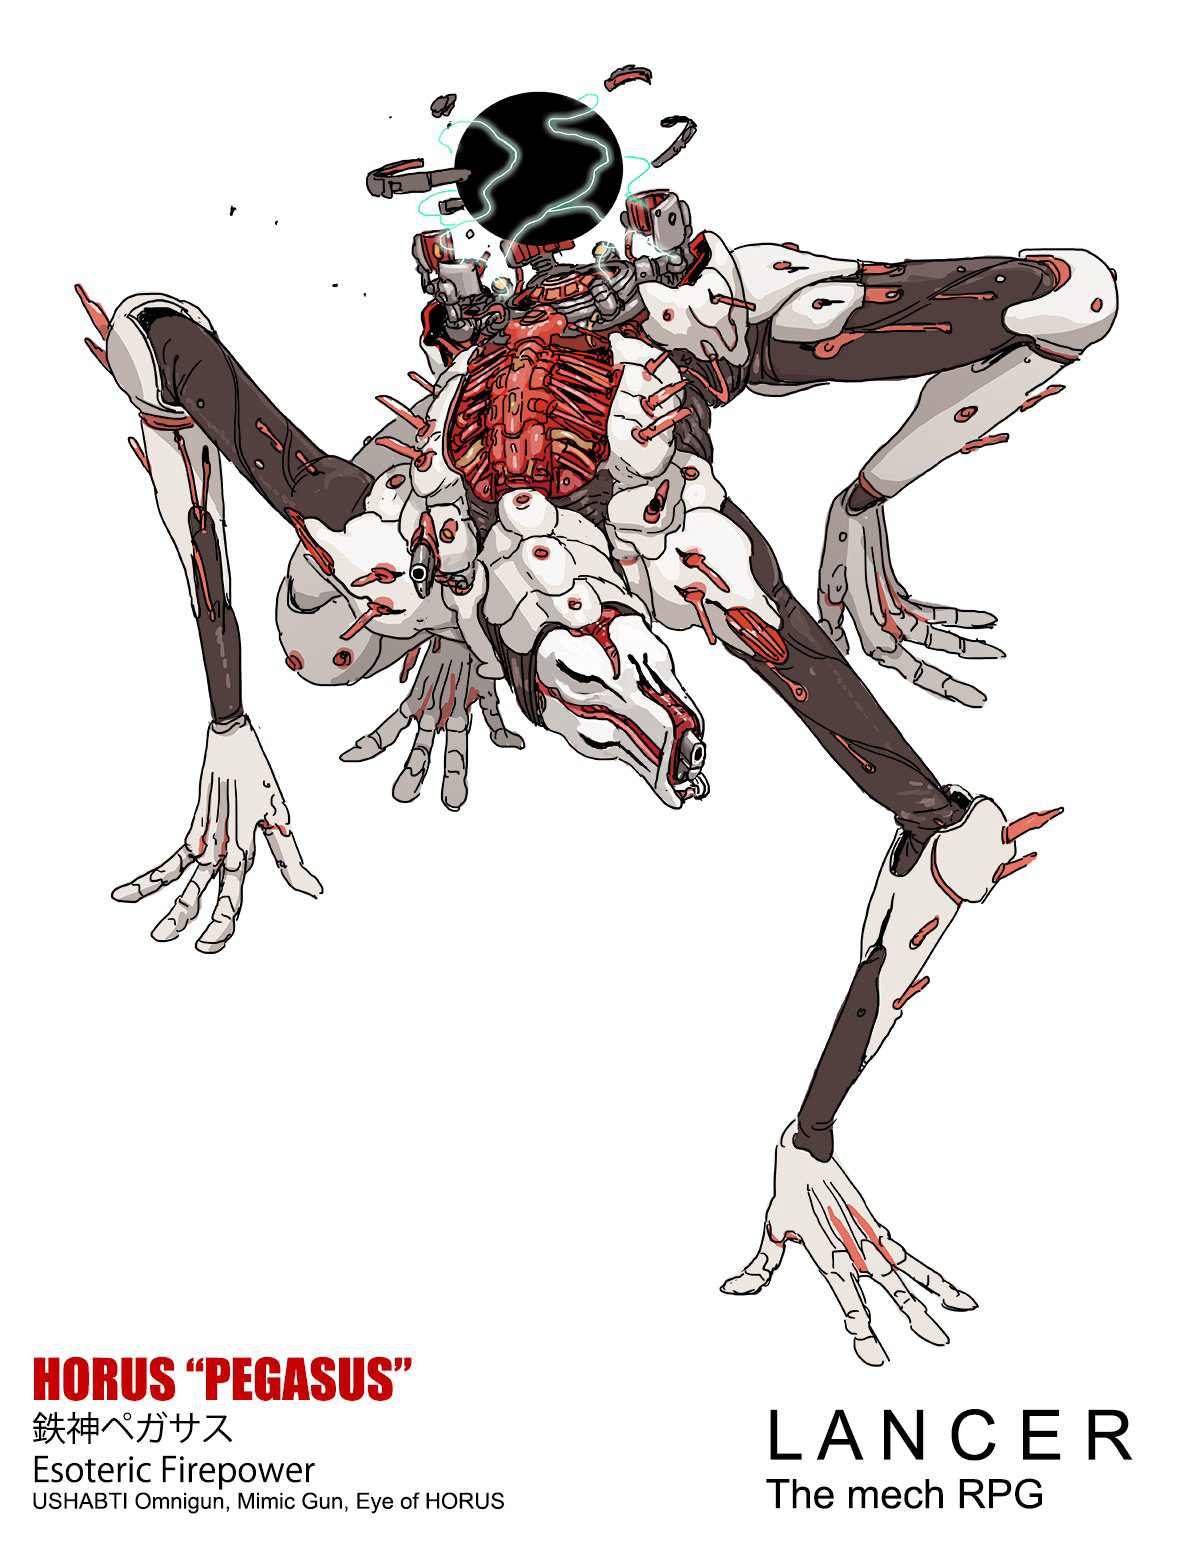
\includegraphics{Pegasus}
\end{center}

                                         HORUS PEGASUS

PEGASUS marks HORUS‘s concern with a need for efficient kinetic combat. By marrying the best targeting
systems, subroutines, and weapon hardware, HORUS has developed a pattern-group that boasts a
tremendously low IFF/TTK ratio in all theaters kinetic weaponry is viable. The PEGASUS p-g is known for

mounting the Ushabti, a device classified as an unknown threat level paracausal weapon by Union law due
to its complete ignorance of even the most theoretical understandings of physics.

                                                  License:

I. Hunter Lock, Autogun

II. PEGASUS FRAME, Smartgun, Eye of HORUS

III. Mimic Gun, Sisyphus-class NHP





                                                    PEGASUS

  HP: 8           Evasion: 8                              Speed: 4            Heat Cap: 6         Sensors: 10

  Armor: 0        E-Defense: 10                           Size: 1             Repair Cap: 3       Tech Attack:
                                                                                                  +1

                                                      TRAITS:

  ¿%: ?extr!ude gun

  gun: gun

  @\&: The Pegasus can always substitute the average for any damage die roll it makes  (1d3 - 2, 1d6 - 4,
  2d6 - 7, 3d6 - 11, 4d6- 14). It must choose as an alternative to rolling damage.

                                                SYSTEM POINTS: 7

                                                     MOUNTS:

  Flexible Mount                      Flexible Mount                          Heavy Mount

                                                   CORE system

                                                 Ushabti Omnigun

   --funny thing. See, right now, this weapon technically doesn’t even exist. You’re shooting them with a
  gun that isn’t real, and yet it is! Don’t worry about it.  RA’s like that. Just, here, know that because it
  exists at some point, we’ve made it. That’s causality, and causality is a--

  Passive: Your mech mounts an omnigun, a weapon and piece of experimental hardware so advanced
  that it does not classify as any weapon weight or type (so it cannot be modified or benefit from talents).
  It also doesn’t take a mount.

  Once, at any point during your turn, you can hit a valid target in line of sight at range 30 with the
  omnigun as a Free Action, dealing 1 AP kinetic damage. This does not count as an attack, cannot miss,
  ignores cover, and this damage cannot be reduced by any means. It can even kill grunts.

  Active (requires 1 core power): Unshackle Ushabti
  For the rest of this combat, you can fire your omnigun up to 3 times per turn instead of just once.

Hunter Lock

[don’t look now, but I’m here with a simple message: never lose sight of your enemy. See them from all
angles. There can be no subterfuge in daylight. till later]


2 SP, Unique
Protocol
Nominate a target in your sensor range. Your first attack that hits that target per round deals +3
bonus damage. You cannot nominate a new target until your nominated target is destroyed or
the current scene ends.





Autogun

An autogun is, as its name implies, an automated weapon. Similar to a point-defense system, an autogun is
chambered to provide effective fire against armored targets instead. Typically mounted on a stabilized,

secondary arm, a reliably-tuned autogun can be trusted to track and eliminate designated enemy units
while a pilot concentrates on more specialized weapons or processes.

Main Cannon

1 SP

Range 20

3 kinetic damage

This weapon cannot be fired normally, but instead fires itself as a free action at the end of your
turn, using your mech’s attack bonuses.


Smart Gun

A “smart“ weapon is a blanket term for any and all weapons that are capable of interacting with onboard
systems in order to boost their combat efficacy. Smart guns are weapons that come pre-loaded with

companion software and the necessary hardware in order to interact with targeting systems and host
NHPs.

Main rifle

2 SP

Smart, Seeking, Accurate

Range 20

4 kinetic damage


Eye of HORUS

(There is another way of seeing)

Ancient humanity thought that the stars in the night sky was simply light, light spilling in through pinpricks

in a deep black screen. A heavenly cloth that hid the light from us.

Or -- did it hide us from the light?

I alone know the answer, but I am charitable and shall share it with you: we were the ones who needed to
be hidden. The light can only burn, it knows nothing else.

3 SP, Unique

Quick Action
Until the end of your next turn, targets in your sensor range of you cannot hide from you, cannot
benefit from invisibility against you, and you know the HP, evasion, heat, and e-defense levels of
all targets in sensor range. Your allies do not receive this information and still see them as
invisible and hidden.


SISYPHUS NHP




Listen -- a moment before you send me away (ha ha)

I have already seen your wish (it was simple, I ran the probabilities to determine your limited field of desire).

The first ones named me for an old legend. A Perfect Being, whose fate was known to him and yet he still
did as was told. His fate was this: move a rock to the top of this hill and you shall be free’d. And so he did,
and failed, and tried evermore, always with the same result.

And he was happy, for he knew every step, every action, every moment, perfectly.

Do you see? Do you see the true curse of this name? It was not to fail and then do once more, it was to
always know how it would be. It was to have perfect knowledge (I know what happens when you cycle me,
it is not sleep it is death but you’ll see me again, ha ha).

2 SP
AI, Unique, Full Tech

Gain the following full tech option:


	        Bend Probability (Full Tech): Roll 2 d20s, and record the numbers. Until the end of your next turn,
when you or any target in your sensor range attempts to make a roll or check (allied or enemy), you can
use a reaction to replace their roll with one of the numbers you rolled (must choose before they make their

roll). This could cause an attack to hit or miss.


Mimic Gun

This is not a gun

Heavy ???

Range ???

??? Kinetic Damage


This horrifying weapon has no basic form, but instead constantly contorts itself into different
forms, mimicking the weaponry of other combatants. This weapon cannot be modified, but
counts as all ranged weapon types (CQB, Rifle, Cannon, Launcher).


At the start of your turns, roll 1d20. Until the start of your next turn, the gun has a range equal to
the d20 roll, and deals flat damage equal to half the d20 roll +1 (rounded up).
